\documentclass[a4paper,english,russian]{G2-105}
\usepackage{standalone}
%    \usepackage{listings}
%    \usepackage{graphicx}
%    \usepackage{longtable}
%    \usepackage{booktabs}
%    \usepackage{newclude}
%    \usepackage[final]{pdfpages}
%    \usepackage{multirow}
%    \usepackage{sansmath} % Enables turning on sans-serif math mode, and using other environments
%    \sansmath % Enable sans-serif math for rest of document
%    \usepackage[math]{blindtext}

%\usepackage[utf8]{luainputenc}
\VSTUSetDocumentNumbersPrefix{}
\VSTUSetDocumentCode{ВРБ-40-461-806-10.19-09.03.04-02-15}
\VSTUSetDocumentTypeDative{выпускной работе бакалавра}
%\VSTUSetDocumentTypeGenitive{выпускную работу бакалавра}
\VSTUSetInitialData{задание, выданное научным руководителем с кафедры ПОАС,
утвержденное приказом ректора}
\VSTUSetPZContents{
    \begin{VSTUList}
    \ulitem{Введение}
    \ulitem{1 Исследование подходов, методов и средств обработки естесвенных языков}
    \ulitem{Цель и задачи исследования}
    \ulitem{2 Исследование грамматики английского языка}
    \ulitem{Выводы}
    \ulitem{3 Разработка метода определения перечислений в английском языке на основе синтаксического анализа}
    \ulitem{Выводы}
    \ulitem{4 Реализация и интеграция метода в плагин Correct Writing, эксперемент, оценка достижения цели}
    \ulitem{Выводы}
    \ulitem{Заключение}
    \ulitem{Список использованных источников}
    \ulitem{Приложение A - Техническое задание}
    \end{VSTUList}
}
\VSTUSetPZGraphics{
    \begin{VSTUNumberedList}
    \ulitem{1: Название работы}
    \ulitem{2-3: Актуальность}
    \end{VSTUNumberedList}
}

\begin{document}
\VSTUSetOrder{1529–ст}{17}{октября}{2014}
\VSTUSetFaculty{Электроники и вычислительной техники}
\VSTUSetDepartment{Программное обеспечение автоматизированных систем}
\VSTUSetDepartmentCode{10.19}
\VSTUSetDirection{09.03.04 Программная инженерия}
\VSTUSetHeadOfDepartment{Зав. кафедрой ПОАС}{д.т.н., проф.}{А. М. Дворянкин}{Дворянкин Александр Михайлович}
\VSTUSetDirector{доц. каф. ПОАС}{к.т.н}{О. А. Сычев}{Сычев Олег Александрович}
%\VSTUSetFacilityExpert{}{}{}{}
\VSTUSetStandardsAdviser{ст. преп. каф. ПОАС}{}{О. Н. Ляпина}{Ляпина Ольга Николаевна}
\VSTUSetStudent{ПрИн-466}{В. А. Клевцов}{Клевцов Вадим Александрович}
\VSTUSetTitle{Поддержка перечислений для языка С++ в типе вопроса CorrectWriting}
\VSTUSetTitleEng{Support enumerations for C++ programm language in the question type CorrectWriting}
%\VSTUAddChapterWordToTOC % обязательно для ПЗ в магистерских диссертациях
\VSTUInitializePZ
%\newpage
\tableofcontents
\newpage
\documentclass{standalone}
% Load any packages needed for this document
\begin{document}
\starchapter{Введение}
% Your document or picture
\end{document}

\newpage
\documentclass{standalone}
% Load any packages needed for this document
\begin{document}
\chapter{Анализ современного состояния проблем в области автоматизированной обработки текстов
на естественных языках}%Исследование подходов, методов и средств обработки естественных языков}
\ttl
\section{Существующие подходы к обработке текстов на естественных языках}
\par В наше время обработка естественных языков используется в нескольких направлениях:
\begin{enumerate}
    \item машинный перевод;
    \item информационный поиск;
    \item реферирование текста;
    \item рубрицирование тектса;
    \item обучение языку и др.
\end{enumerate}
\par Несмотря на обилие направлений использования, подходов к обработке всего четыре, символьный, вероятностный, установления связей и гибридный.
\section{Символьный подход}
\par Подход основанный представлении языка как модели сложной, но прозрачной. Примерами такой модели могут послужить:
\begin{enumerate}
    \item обучение на правилах;
    \item индуктивное логическое программирование;
    \item деревья разрешений;
    \item концептуальная кластеризации;
    \item алгоритмы типа k-средних.
\end{enumerate}
\par Более подробно перечисленные методы будут описаны ниже. Общей чертой данных моделей является способ их получение, а именно обучение.
\subsection{Обучение на правилах} % (fold)

\par Один из старейших методов обучение и построения моделей. Используется в случаях когда правила не возможно закодировать правила иначе, то есть когда правила являются эвристическими.

\subsection{Индуктивное логическое программирование} % (fold)

\par Это раздел машинного обучения использующий в качестве примеров, фоновых знаний и гипотез логическое программирование. Логическое программирование — это парадигма программирования, которая основана на автоматическом доказательстве теорем. Логическое программирование основано на теории и аппарате математической логики с использованием математических принципов резолюций.

\subsection{Деревья разрешений} % (fold)

\par Это средство принятия решений, используемое в прогнозировании и обработке данных. Структура дерева представляет собой «листья» и «ветки». На ребрах («ветках») дерева решения записаны атрибуты, от которых зависит целевая функция, в «листьях» записаны значения целевой функции, а в остальных узлах — атрибуты, по которым различаются случаи. Для определения значения, необходимо спуститься по дереву до листа и вернуть его значение.

\subsection{Концептуальная кластеризация} % (fold)

\par Кластеризация является еще одним способом обработки естественных языков. Кластеризация является задачей обучения без учителя. Суть метода заключается в обучении на большой выборке, позволяющий выделить объекты в однородные группы. Ниже приведена классификация методов кластеризации являющаяся общепринятой:
\begin{enumerate}
    \item вероятностный подход:
        \begin{enumerate}
            \item метод К-средних;
            \item метод К-medians;
            \item EM-алгоритм;
            \item алгоритм семейства FOREL;
            \item дискриминантный анализ,
        \end{enumerate}
    \item методы на основе систем искусственного интеллекта:
        \begin{enumerate}
            \item метод нечеткой кластеризации С-средних;
            \item нейронная сеть Кохонена;
            \item генетический алгоритм,
        \end{enumerate}
    \item логический подход. Кластеризация на основе дерева решений,
    \item теоретико-графический подход:
        \begin{enumerate}
            \item графические алгоритмы кластеризации;
        \end{enumerate}
    \item иерархический подход. Используется в ситуации наличия подгрупп внутри групп:
        \begin{enumerate}
            \item агломеративные алгоритмы;
            \item дивизивные алгоритмы,
        \end{enumerate}
    \item остальные методы:
        \begin{enumerate}
            \item статистические методы кластеризации;
            \item ансамбль кластеров;
            \item алгоритмы семейства KRAB;
            \item алгоритм, основанный на методе просеивания DBSCAN и др.
        \end{enumerate}
\end{enumerate}

\subsection{Алгоритмы типа k-средних} % (fold)

\par Наиболее популярный алгоритм кластеризации, стремящийся минизировать суммарное квадратичное отклонение точек кластеров от центров этих кластеров.
\par Основная идея заключается в том, что на каждой итерации вычисляется центр масс для каждого кластера, полученного на предыдущем шаге, затем векторы разбиваются на кластеры вновь в соответствии с тем, какой из новых центров оказался ближе по выбранной метрике.
\par Алгоритм завершается, когда на какой-то итерации не происходит изменения центра масс кластеров. Это происходит за конечное число итераций, так как количество возможных разбиений конечного множества конечно, а на каждом шаге суммарное квадратичное отклонение не увеличивается, поэтому зацикливание невозможно.

% subsection  (end)
% subsection  (end)
% subsection  (end)
% subsection  (end)
% subsection  (end)
% subsection  (end)
\section{Вероятностный подход}
\par Подход использует различные математические техники, а также большие текстовые корпуса для разработки обобщенных моделей языковых явлений, базой для которой является реальные примеры найденные в текстовом корпусе не используя дополнительных знаний о языке или о внешнем мире. Основное отличие от символьного подхода использование реальных данных в качестве первичного источника информации.
\par В вероятностном подходе существует несколько течений, среди которых особого внимания заслуживают модели, максимизирующие энтропию и скрытые марковские модели (СММ). СММ  это конечный автомат, который имеющий множество состояний с определенными вероятностями переходов между ними. Каждое состояние производит один из наблюдаемых результатов с определенной вероятностью. Хотя результаты являются видимыми, но состояние модели скрыто от внешнего наблюдения. Главным преимуществом вероятностных моделей заключено в том, что они дают способ решения многих видов неоднозначных проблем, формулируемых так "с учетом N некоторых неоднозначных вводов выбрать один наиболее вероятный".

\subsection{Методы максимизации энтропии} % (fold)

\par Данный метод классификации основан на понятии информационной энтропии. Информационная энтропия - это мера неопределенности вероятностного распределения.
\par \textbf{Еще не нашел хорошего описания этого алгоритма.}

\subsection{Скрытые макрковские модели} % (fold)
\par Скрытая марковская модель — статистическая модель, имитирующая работу процесса, похожего на марковский процесс с неизвестными параметрами, и задачей является определение неизвестных параметров на основе наблюдаемых. Полученные параметры могут быть использованы в дальнейшем анализе.

% subsection  (end)
% subsection  (end)
\section{Подход установления связей}
\par Подход установление связей основан на моделях массивных связанных наборов простых и нелинейных компонентов. Эти компоненты работают параллельно. Приобретенное в результате обработки знание сохраняется в образце весов взаимосвязи компонентов.
\section{Гибридный подход}
\par Гибридные методы используют преимущества трех только что описанных подходов, минимизируя человеческие усилия, требуемые для типовой лингвистической конструкции и максимизируя гибкость, эффективность, и надежность применения NLP при человеко-компьютерном взаимодействии.

\par При всех подходах обработка языка, как правило, включает элементы машинного обучения: модель классификации и обучающую последовательность. На основании описания атрибутов каждого объекта модель классификации относит каждый объект в какой-то класс, обучающая последовательность ставит в соответствие последовательности объектов последовательность классов.

\section{Выбор программного средства синтаксического анализа}

\par Синтаксический анализ является сложным и трудоемким процессом, в особенности если речь идет об анализе естественного языка. Именно это стало причиной принятия решения о использовании стороннего средства синтаксического анализа.
\par Было рассмотрено множество синтаксических анализаторов и выделены критерии сравнения. Наиболее развитыми на момент написания диссертации являются следующие анализаторы:
\begin{enumerate}
    \item анализатор Стенфорского университета;
    \item анализатор Института Брауна;
    \item анализатор Института Беркли;
    \item анализатор Института Токио.
\end{enumerate}
\subsection{Критерии сравнения}
\par От выбора критериев сравнения зависит решения о выборе средства синтаксического анализа, что в конечном итоге повлияет на результат все проделанной работы.
\par Moodle является системой управления обучением с открытым исходным кодом, что накладывает ограничения на используемое с ним программное обеспечение. Поэтому лицензия средства синтаксического анализа является важным критерием отбора. Каждый из рассматриваемых средств синтаксического анализа имеет открытую лицензию, которая позволяет использовать это средство в связке с Moodle.
\par Следующим важным критерием отбора является наличие тестов для выбираемого программного средства. Так как наличие большого количества тестов и покрытие этими тестами кода, указывает на качество программного средства, а так же позволяет оценить его функциональные возможности.
\par Определение части речи, к которой принадлежит лексема, является минимальной необходимой функциональностью для использования для определения перечислений в тексте написанном на естественном языке. Наличие этого критерия является обязательный требованием к программному средству синтаксического анализа.
\par Еще одним критерием сравнения является язык на котором написано программное средство. Этот критерий повлияет на системные требования предъявляемые разрабатываемым программным средством.
\par Одним из важных критериев является способ взаимодействия разрабатываемого программного средства со средством синтаксического анализа.
\par В качестве дополнительного критерия выступает возможность определение средством синтаксического анализа связей между лексемами в предложении.

\subsection{Синтаксический анализатор Института Брауна}

\par Данный синтаксический анализатор разрабатывается начиная с 2000 года. И сильно изменился с первой версии. Это синтаксический анализатор основанный на методе максимизации энтропии и модели самообучения. Данное программное средство разработано на языке Python и предполагает использование по средствам вызова из командной строки. К исходному коду парсера прилагается набор тестов, позволяющих оценить качество написанного программного средства.
\par Возможности данного пасера ограничиваются определением членов предложения и принадлежащих им лексем.

\subsection{Синтаксический анализатор Института Беркли}

\par Данное программное средство разрабатывается Институтом Беркли с 2001 года. В основу парсера лег символьный подход к синтаксическому анализу, алгоритм К-best. Данное программное средство написано на языках Java и Scala. И так же как рассмотренное ранее средство синтаксического анализа предполагает запуск с аргументами из командной строки.
\par Возможности данного парсера аналогичны возможностям ранее рассмотренного программного средства.

\subsection{Синтаксический анализатор Института Токио}

\par Институт Токио занимается разработкой средства синтаксического анализа английского языка с 2005 года. Программное средство использует подход установления связей в процессе анализа текста, алгоритм построения структуры предложения управляемой главным членом предложения. Язык написания данного программного средства C++. В отличие от двух предыдущих средств синтаксического анализа данное помимо запуска из командной строки предлагает возможность запуска в качестве сервера, с которым возможно общение по протоколу HTTP.
\par Возможности данного средства синтаксического анализа расширяют возможности средств описанных выше, за счет определения связей между членами предложения.

\subsection{Синтаксический анализатор Стэнфордского университета}

\par Данное средство синтаксического анализа естественных языков ведет свою историю с 1990 года. Этот синтаксический анализатор является самым развитым на данный момент. Данное программное средство использует гибридный подход к синтаксическому анализу. В качестве языка написания данного программного средства выступает язык Java. Тестовая база данного синтаксического анализа включается в себя более 10000 тестов. Так же как и предыдущий анализатор данный предлагает два режима работы, в качестве средства командной строки, а так же в качестве отдельного сервера, с возможность выполнения запроса к нему по протоколу HTTP.
\par Возможности данного программного средства синтаксического анализа аналогичны возможностям предыдущего средства. С одной лишь разницей, данное средство имеет более высокие показатели качества за счет использования более продвинутого подхода к синтаксическому анализу.

\subsection{Выводы}

\par В результате изучения представленных выше программных средств синтаксического анализа, было принято решение выбрать для использование программное обеспечение разработанное на базе университета Стенфорда. Причинами для такого решения послужили следующие аргументы:
\begin{enumerate}
    \item синтаксический анализатор Стенфорского университета использует обобщенное описание синтаксиса языка, что позволяет использовать его с другими естественными языками;
    \item это наиболее активно развивающийся синтаксический анализатор;
    \item данный анализатор имеет наибольшую тестовую базу, что позволяет удостовериться в качестве его работы на наибольшем количестве тестовых ситуаций.
\end{enumerate}

\end{document}

\documentclass{standalone}
% Load any packages needed for this document
\begin{document}
% Your document or picture
\chapter{Выделение структур английского языка удовлетворяющих перечислениям}%Исследование грамматики английского языка}
\ttl
\section{Определение структур языка являющихся перечислениями}
\par Для построения модели перечисления в контексте естественного языка, необходимо определить структуры языка подходящие на роль перечислений. В естественных языках перечислениями являются однородные члены предложения, а также сложно сочиненные члены предложения.
\par В английском языке существуют следующие однородные члены предложения:
\begin{enumerate}
    \item сказуемые;
    \item подлежащие;
    \item определения;
    \item дополнения;
    \item обстоятельства.
\end{enumerate}
\par Рассмотрение каждой структуры в отдельности позволит построить модель перечисления на естественном языке, и выработать алгоритм определения перечислений для естественного языка.
\subsection{Сказуемое} % (fold)
% описание
% пример
% используемое правило
% 
\par Сказуемое является главным членом двусоставного предложения, обозначающим действие или признак того, что выражено подлежащим.
\par Сказуемое имеет лексическое значение (именует то, что сообщается о реалии, названной в подлежащем) и грамматическое значение (характеризует высказывание с точки зрения реальности или ирреальности и соотнесенности высказывания с моментом речи, что выражается формами наклонения глагола, а в изъявительном наклонении — и времени).
\par Рассмотрим как пример следующее предложение: <<We went to the cafe and buy a cup of coffee.>>. Для большей наглядности используем изображение ~\ref{skazuemoe}.
\begin{figure}
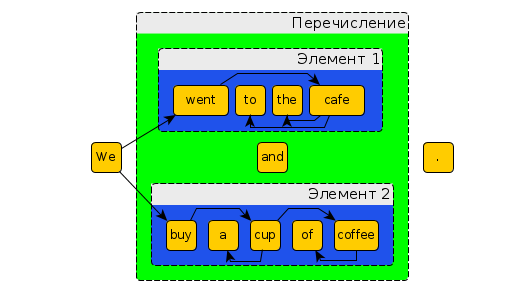
\includegraphics[width=\textwidth]{images/sentences2.png}
\label{skazuemoe}
\caption{Предложение с однородными сказуемыми, осложнеными зависимыми членами предложения}
\end{figure}
\begin{figure}
    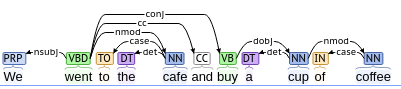
\includegraphics[width=\textwidth]{images/sentences21.png}
\label{skazuemoe2}
\caption{Предложение с однородными сказуемыми, осложнеными зависимыми членами предложения}
\end{figure}
\par На рисунке ~\ref{skazuemoe} выделены элементы перечисления, и стрелками показаны важные для нас отношения членов предложения. От подлежащего <<We>> две стрелки идут к однородным членам <<went>>  и <<buy>> , осложненым обстоятельством места и дополнением связи с ними также показаны на рисунке. На рисунке ~\ref{skazuemoe2} представлено дерево построенное Стенфорским парсером для данного предложения, оно выглядит иначе, основынм отличием является то что он подлежащего построена связь только к первому однородному сказуемому, в свою очередь существует связь соединяющая однородные члены между собой. Специфика построения синтаксических деревьев будет учтена при создании модели перечисления.
\subsection{Подлежащее} % (fold)
\par Подлежащее называет то, о ком или о чём говорится в предложении. Подлежащие не разрывно связано со сказуемым. Рассмотрим в качестве примера следующее предложение: <<Hot coffee and green tea the are best monday morning drinks.>>. Связи элементов представлены на рисунке ~\ref{podlezhachie}, в данном случае два однородных подлежащих <<coffee>> и <<tea>> , осложненные определениями, связаны со сказуемым <<are>> . На рисунке ~\ref{podlezhachie2} изображено посттроенное дерево. Тут как и в первом случае присутсвуют отличия, демонстрирующие отличие логического подхода построения связей между элементами от лингвистического подхода синтаксического подхода. Данное различие так же необходимо учесть при создании модели.

\begin{figure}[!ht]
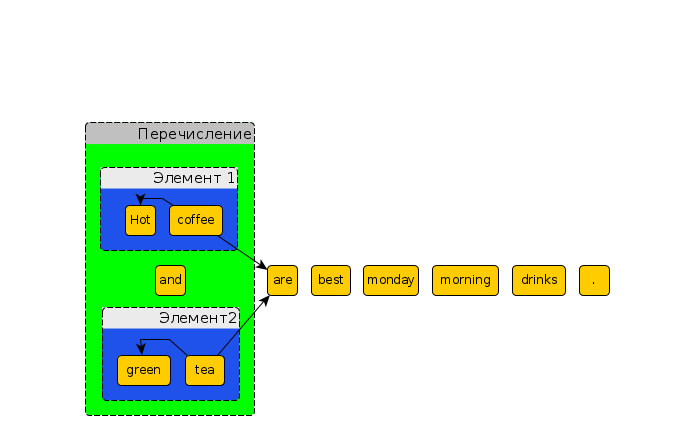
\includegraphics[width=\textwidth]{images/sentences1.png}
\label{podlezhachie}
\caption{Предложение с однородными подлежащими, осложнеными зависимыми членами предложения}
\end{figure}
\begin{figure}[!ht]
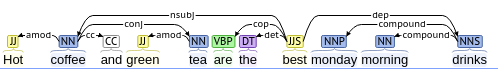
\includegraphics[width=\textwidth]{images/sentences11.png}
\label{podlezhachie2}
\caption{Предложение с однородными подлежащими, осложнеными зависимыми членами предложения}
\end{figure}
\newpage
\subsection{Определение} % (fold)
\par Определение — второстепенный член предложения, обозначающий признак, качество, свойство предмета. Рассмотрим на примере следующего предложения <<The weather today is a little cloudy, extremely raining, freezing-cold and densy foggy.>>. На рисунке ~\ref{opredelenie} представлены члены предложения и важные для исследования связи между ними. Связи отвечающие за однородные члены идут от лексеммы <<weather>> к лексеммам являющихся определениями <<cloudy>>, <<raining>>, <<freezing-cold>> и <<foggy>>, так же как и в примерах выше присутствуют зависимые лексемы. Результат определния связей между лексемами представлен на рисунке ~\ref{opredelenie2}, прослеживается общая для каждого из примеров логика, что связь между подлежащим и однородными определениями парсер представляет в виде связей двух видов: 
\begin{enumerate}
    \item связь подлежащего и первого из однородных определений;
    \item связи между первым и остальными определниями.
\end{enumerate}

\begin{figure}[!ht]
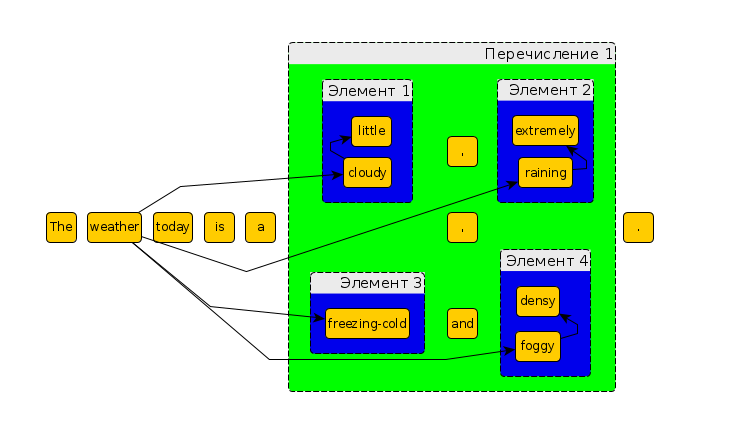
\includegraphics[width=\textwidth]{images/sentences7.png}
\label{opredelenie}
\caption{Предложение с однородными определениями}
\end{figure}
\begin{figure}[!ht]
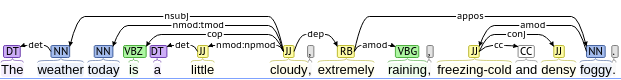
\includegraphics[width=\textwidth]{images/sentences71.png}
\label{opredelenie2}
\caption{Предложение с однородными определениями}
\end{figure}
\subsection{Дополнение} % (fold)
% описание
% пример
% используемое правило
%
Дополнение — второстепенный член предложения, выраженный существительным или местоименным существительным. Дополнение обозначает предмет или лицо, являющееся объектом действия, выраженного сказуемым.
We need your first and last names, back-white photo and home and mobile number.
\begin{figure}[!ht]
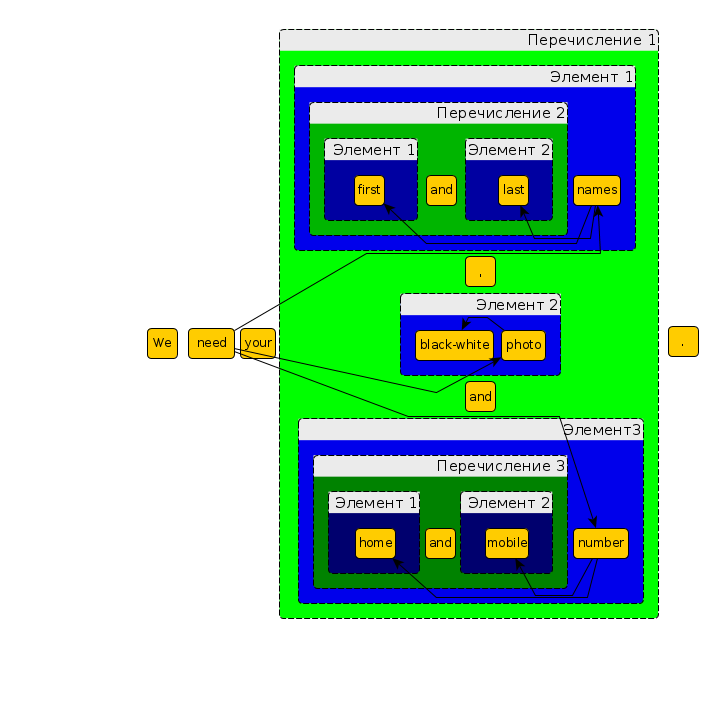
\includegraphics[width=\textwidth]{images/sentences6.png}
\label{obstoyatelstvo}
\caption{Предложение с однородными сказуемыми, осложнеными зависимыми лексемами}
\end{figure}
\newpage
\subsection{Обстоятельства} % (fold)
% описание
% пример
% используемое правило
%
I go to the cinema, cafe and to the park.
\begin{figure}[!ht]
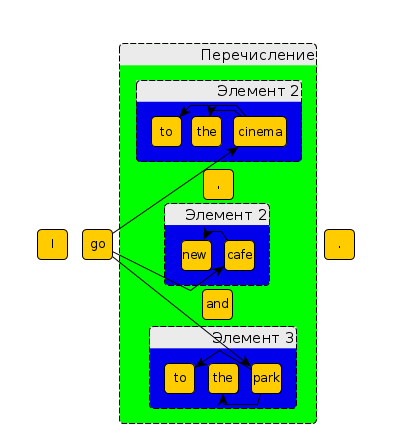
\includegraphics[width=\textwidth]{images/sentences3.png}
\label{obstoyatelstvo}
\caption{Предложение с однородными сказуемыми, осложнеными зависимыми лексемами 1}
\end{figure}
\newpage
\subsection{Сложносочиненые предложения} % (fold)
% описание
% пример
% используемое правило
%
I see a big group of people which contains three subgroups: children, women and men, who were dressed in blue overalls or strange suits with red and green lines.

\begin{figure}[!ht]
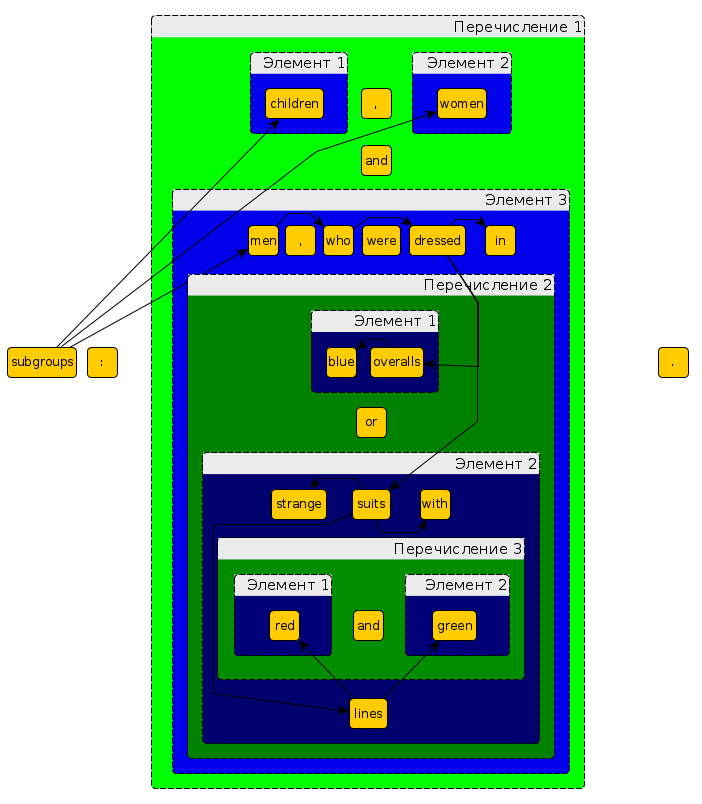
\includegraphics[width=\textwidth]{images/sentences5.png}
\label{sss}
\caption{Предложение с однородными сказуемыми, осложнеными зависимыми лексемами}
\end{figure}
\newpage
\section{Построение модели}
%
\par 
\end{document}

\documentclass{standalone}
% Load any packages needed for this document
\begin{document}
% Your document or picture
\end{document}

\documentclass{standalone}
% Load any packages needed for this document
\begin{document}
% Your document or picture
\end{document}

\newpage
\documentclass{standalone}
\begin{document}
\begin{thebibliography}{1}

% 2 источника по максимизации энторопии
\bibitem{1} Найденова К. А. , Невзорова О. А. , Машинное обучение в задачах обработки естественного языка: Обзор современного состояния исследований / К. А. Найденова, О. А. Невзорова; Ученые записки Казанского государственного университета. Физико-математические науки. - Казань, 2008. - Том 150, книга 4, 20 c.
\bibitem{2} Аматов, А.М. Информационная энтропия как фактор конвергенции синтаксических структур в язуках разных типов( на примере русского и английского языков) / А. М. Аматов // Вест. Волгогр. гос. ун-та, Сер. 2, Языкозн. / ВолГУ. - Волгоград - №2 - С. 142-146
% 1 по скрытой марковской модели
\bibitem{3} Gernot A. Fink, Markov Models for Pattern Recognition: From Theory to Applications / Gernot A. Fink; Springer Berlin Heidelberg. - Berlin, 2007. - 248 p.
% 2 по концептуальной класстеризации
\bibitem{4} Кластеризация [Electronic resource]. – Mode of access : http://www.machinelearning.ru/wiki/index.php?title=%D0%9A%D0%BB%D0%B0%D1%81%D1%82%D0%B5%D1%80%D0%B8%D0%B7%D0%B0%D1%86%D0%B8%D1%8F 
(date of access 12.03.2015).
\bibitem{5} Бериков В. С., Лбов Г. С. Современные тенденции в кластерном анализе // Всероссийский конкурсный отбор обзорно-аналитических статей по приоритетному направлению «Информационно-телекоммуникационные системы», 2008. — 26 с.
% 1 про деревья разрешений
\bibitem{6} Quinlan, J. R., (1986). Induction of Decision Trees. Machine Learning 1: 81-106, Kluwer Academic Publishers
% 1 к средних
\bibitem{7} Adam Coates and Andrew Y. Ng. Learning Feature Representations with K-means, Stanford University, 2012
% 1 индукционное логическое программирование
\bibitem{8} Девятков В. В. Системы искусственного интеллекта / Гл. ред. И. Б. Фёдоров. — М.: Изд-во МГТУ им. Н. Э. Баумана, 2001. — 352 с.
% Институт Беркли
\bibitem{9} Pauls A. , K-Best A\(\ast\) Parsing. / A. Pauls, D. Klein; University of California, Berkeley. - California, 2009. - 9 p.
\bibitem{10} Durrett G. , Neural CRF Parsing. / G. Durrett, D. Klein; University of California, Berkeley. - California, 2015. - 11 p.
\bibitem{11} Liang P. , Agreement-Based Learning. / P. Liang, D. Klein, M. I. Jordan; University of California, Berkeley. - California, 2008. - 8 p.
\bibitem{12} Petrov S. , Improved Inference for Unlexicalized Parsing. / S. Petrov, D. Klein; University of California, Berkeley. - California, 2007. - 8 p.
\bibitem{13} Durrett G. , Learning-Based Single-Document Summarization with Compression and Anaphoricity Constraints. / G. Durrett, T. Berg-Kirkpatrick, D. Klein; University of California, Berkeley. - California, 2016. - 11 p.

% Иститут Токио
% Иститут Стенфорда
% Гугл
% 2-3 учебника части речи

\end{thebibliography}
\end{document}

\end{document}
